\documentclass[12pt,oneside]{report}
%%%%%%%%%%%%%%%%%%%%%%%%%%%%%%%%%%%%%%%%%%%%%%%%%%%%%%%%%%%%%%%%%%%%%%%%%%%%%%%
\input{preambule_2018}
%%%%%%%%%%%%%%%%%%%%%%%%%%%%%%%%%%%%%%%%%%%%%%%%%%%%%%%%%%%%%%%%%%%%%%%%%%%%%%%
\portrait
%\paysage
%%%%%%%%%%%%%%%%%%%%%%%%%%%%%%%%%%%%%%%%%%%%%%%%%%%%%%%%%%%%%%%%%%%%%%%%%%%%%%%

%entête classique

\fancypagestyle{garde_tete}{% 
%\fancyhead[C]{\small\textbf{\seconde} \hfill \small \textbf{Année 2015-2016}}
\renewcommand{\headrulewidth}{0cm}}

\newcommand{\tete}{
\thispagestyle{garde_tete}
\chapitre{Exemples de graphes}
\noindent 
\vspace{-1em}
}

%%%%%%%%%%%%%%%%%%%%%%%%%%%%%%%%%%%%%%%%%%%%%%%%%%%%%%%%%%%%%%%%%%%%%%%%%%%%%%%
%%%%%%%%%%%%%%%%%%%%%%%%%%%%%%%%%%%%%%%%%%%%%%%%%%%%%%%%%%%%%%%%%%%%%%%%%%%%%%%
%\tikzset{domaine/.style 2 args={domain=#1:#2}}

%utilise le package tcolorbox
\newtcolorbox{mybox}[2][]{colback=red!5!white,
colframe=red!75!black,fonttitle=\bfseries,
colbacktitle=red!85!black,enhanced,
attach boxed title to top left={xshift=2mm,yshift=-2mm},
title=#2,#1}

\newtcolorbox{module}[2][]{colback=red!5!white,
colframe=red!75!black,fonttitle=\bfseries,
colbacktitle=red!85!black,enhanced,
attach boxed title to bottom right={xshift=-5mm,yshift=+2mm},
title=#2,#1}
%%%%%%%%%%%%%%%%%%%%%%%%%%%%%%%%%%%%%%%%%%%%%%%%%%%%%%%%%%%%%%%%%%%%%%%%%%%%%%%
%%%%%%%%%%%%%%%%%%%%%%%%%%%%%%%%%%%%%%%%%%%%%%%%%%%%%%%%%%%%%%%%%%%%%%%%%%%%%%%

%%%%%%%%%%%%%%%%%%%%%%%
%% DEBUT DU DOCUMENT %%
%%%%%%%%%%%%%%%%%%%%%%%

\begin{document}
%\selectlanguage{english}
\selectlanguage{french}
\setlength\parindent{0mm}
\tete 		%entête classique

\renewcommand \footrulewidth{0.2pt}%
\renewcommand \headrulewidth{0pt}%
\pagestyle{fancy}
\fancyhf{}
\pieddepage{}{\thepage / \pageref{LastPage}}{}

%%%%%%%%%%%%%%%%%%%%%%%%%%%%%%%%%%%%%%%%%%%%%%%%%%%%%%%%%%%%
\begin{spacing}{1.2}
%%%%%%%%%%%%%%%%%%%%%%%%%%%%%%%%%%%%%%%%%%%%%%%%%%%%%%%%%%%%

%%%%%%%%%%%%%%%%%%%%%%%%%%%%%%%%%%%%%%%%%%%%%%%%%%%%%%%%%%%%%%%%%%%%%%%%%
%%%%%%%%%%%%%%%%%%%%%%%% exercice 1 %%%%%%%%%%%%%%%%%%%%%%%%%%%%%%%%%%%%%
\label{exemple1}
%%%%%%%%%%%%%%%%%%%%%%%%%%%%%%%%%%%%%%%%%%%%%%%%%%%%%%%%%%%%%%%%%%%%%%%%%
\begin{Exemple}[\ 1]{}
\begin{center}
\begin{tikzpicture}
  \SetVertexNormal[Shape      = circle,
                   %FillColor  = yellow,
                   LineWidth  = 1.5pt]
  \SetUpEdge[lw         = 1pt,
             color      = black,
             labelcolor = white,
             labeltext  = red,
             labelstyle = {sloped,draw,text=blue}]
 %\tikzstyle{EdgeStyle}=[bend left]
 \Vertex[x=0, y=0,L={\textbf{G}}]{G}
 \Vertex[x=-2, y=1,L={\textbf{F}}]{F}
 \Vertex[x=-3, y=4,L={\textbf{A}}]{A}
 \Vertex[x=-1, y=5,L={\textbf{B}}]{B}
 \Vertex[x=1, y=4,L={\textbf{C}}]{C}
 \Vertex[x=2, y=2,L={\textbf{D}}]{D}
 \Vertex[x=-2, y=3,L={\textbf{E}}]{E}
 \Edges(A,B,C,F,E,C)
 \Edges(F,A,C)
 \Edges(E,B,D,G,F)
 \Edges(E,C,F)
 \Edges[label={12}](E,D)
\end{tikzpicture}
\end{center}

\end{Exemple}

%%%%%%%%%%%%%%%%%%%%%%%%%%%%%%%%%%%%%%%%%%%%%%%%%%%%%%%%%%%%%%%%%%%%%%%%%
%%%%%%%%%%%%%%%%%%%%%%%% exercice 2 %%%%%%%%%%%%%%%%%%%%%%%%%%%%%%%%%%%%%
\label{exemple2}
%%%%%%%%%%%%%%%%%%%%%%%%%%%%%%%%%%%%%%%%%%%%%%%%%%%%%%%%%%%%%%%%%%%%%%%%%
%%%%%%%%%%%%%%%%%%%%%%%%%%%%%%%%%%%%%%%%%%%%%%%%%%%%%%%%%%%%
%\newpage
\medskip
\begin{Exemple}[\ 2]{}

\begin{center}
\begin{tikzpicture}[scale=5,node distance=4cm]
\GraphInit[vstyle=Shade]
\tikzset{LabelStyle/.style={draw,fill=yellow,text=red}}
\Vertex{A}
\EA(A){B}
\EA(B){C}
\tikzset{node distance=8cm}% modifie la distance entre les nodes
\NO(B){D}
\Edge[label=1](B)(D)
\tikzset{EdgeStyle/.append style = {bend left}}
\Edge[label=4](A)(B)
\Edge[label=5](B)(A)
\Edge[label=6](B)(C)
\Edge[label=7](C)(B)
\Edge[label=2](A)(D)
\Edge[label=3](D)(C)
\end{tikzpicture}
\end{center}
\end{Exemple}

%%%%%%%%%%%%%%%%%%%%%%%%%%%%%%%%%%%%%%%%%%%%%%%%%%%%%%%%%%%%%%%%%%%%%%%%%
%%%%%%%%%%%%%%%%%%%%%%%% exercice 3 %%%%%%%%%%%%%%%%%%%%%%%%%%%%%%%%%%%%%
\label{exemple3}
%%%%%%%%%%%%%%%%%%%%%%%%%%%%%%%%%%%%%%%%%%%%%%%%%%%%%%%%%%%%%%%%%%%%%%%%%
%%%%%%%%%%%%%%%%%%%%%%%%%%%%%%%%%%%%%%%%%%%%%%%%%%%%%%%%%%%%
%\newpage
\medskip
\begin{Exemple}[\ 3]{}

\SetVertexNormal[Shape      = circle,
FillColor  = orange,
LineWidth  = 2pt]
\SetUpEdge[lw               = 1.5pt,
color            = black,
labelcolor       = white,
labeltext        = red,
labelstyle       = {sloped,draw,text=blue}]
\begin{tikzpicture}
\Vertex[x=0 ,y=0]{K}
\Vertex[x=0 ,y=2]{F}
\Vertex[x=-1,y=4]{D}
\Vertex[x=3 ,y=7]{H}
\Vertex[x=8 ,y=5]{B}
\Vertex[x=9 ,y=2]{N}
\Vertex[x=5 ,y=0]{M}
\Vertex[x=3 ,y=1]{S}
\tikzset{EdgeStyle/.append style = {bend left}}
\Edge[label = $120$](K)(F)
\Edge[label = $650$](H)(S)
\Edge[label = $780$](H)(M)
\Edge[label = $490$](D)(B)
\Edge[label = $600$](D)(M)
\Edge[label = $580$](B)(M)
\Edge[label = $600$](H)(N)
\Edge[label = $490$](F)(H)
\tikzset{EdgeStyle/.append style = {bend right}}
\Edge[label = $630$](S)(B)
\Edge[label = $210$](S)(N)
\Edge[label = $230$](S)(M)
\end{tikzpicture}
\end{Exemple}

%%%%%%%%%%%%%%%%%%%%%%%%%%%%%%%%%%%%%%%%%%%%%%%%%%%%%%%%%%%%%%%%%%%%%%%%%
%%%%%%%%%%%%%%%%%%%%%%%% exercice 4 %%%%%%%%%%%%%%%%%%%%%%%%%%%%%%%%%%%%%
\label{exemple4}
%%%%%%%%%%%%%%%%%%%%%%%%%%%%%%%%%%%%%%%%%%%%%%%%%%%%%%%%%%%%%%%%%%%%%%%%%
%%%%%%%%%%%%%%%%%%%%%%%%%%%%%%%%%%%%%%%%%%%%%%%%%%%%%%%%%%%%
%\newpage
\medskip
\begin{Exemple}[\ 4]{}

\begin{tikzpicture}
\GraphInit[vstyle=Shade]
\tikzset{node distance = 4cm}
\Vertex{e}
\NOEA(e){f}
\SOEA(e){d}
\SOEA(f){h}
\Vertex[position={above of=e,yshift=2cm}]{g}
\Vertex[position={left  of=g,xshift=-1cm}]{c}
\Vertex[position={left  of=d,xshift=-2cm}]{a}
\SOWE(c){b}
\tikzstyle{LabelStyle}=[fill=white]
\tikzstyle{EdgeStyle}=[color=red]
\Edge[label=$3$](a)(b)
\Edge[label=$11$](a)(c)
\Edge[label=$6$](a)(e)
\Edge[label=$17$](a)(d)
\Edge[style={pos=.25},label=$20$](a)(g)
\Edge[label=$5$](c)(b)
\Edge[label=$6$](c)(e)
\Edge[label=$7$](c)(g)
\Edge[label=$7$](f)(e)
\Edge[label=$3$](d)(e)
\Edge[label=$9$](d)(h)
\Edge[label=$6$](g)(e)
\Edge[style={bend left,out=45,in=135},label=$11$](g)(h)
\Edge[label=$4$](f)(h)
\end{tikzpicture}
\end{Exemple}

%%%%%%%%%%%%%%%%%%%%%%%%%%%%%%%%%%%%%%%%%%%%%%%%%%%%%%%%%%%%%%%%%%%%%%%%%
%%%%%%%%%%%%%%%%%%%%%%%% exercice 5 %%%%%%%%%%%%%%%%%%%%%%%%%%%%%%%%%%%%%
\label{exemple5}
%%%%%%%%%%%%%%%%%%%%%%%%%%%%%%%%%%%%%%%%%%%%%%%%%%%%%%%%%%%%%%%%%%%%%%%%%
%%%%%%%%%%%%%%%%%%%%%%%%%%%%%%%%%%%%%%%%%%%%%%%%%%%%%%%%%%%%
%\newpage
\medskip
\begin{Exemple}[\ 5]{}

 \begin{tikzpicture}
 \GraphInit[vstyle=Dijkstra]
 \tikzset{node distance = 4cm}
 \Vertices*{square}{B,C,D,A}
 \tikzset{node distance = 2.82cm}
 \NOWE(B){E}
 \NOEA(C){S}
 \Edge[label=$3$](E)(A)
 \Edge[label=$1$](E)(B)
 \Edge[label=$1$](A)(B)
 \Edge[label=$3$](B)(C)
 \Edge[label=$3$,style={pos=.25}](A)(C)
 \Edge[label=$5$,style={pos=.75}](B)(D)
 \Edge[label=$4$](A)(D)
 \Edge[label=$1$](S)(D)
 \Edge[label=$3$](C)(S)
 \Edge[label=$1$](C)(D)
 \end{tikzpicture}
\end{Exemple}

%%%%%%%%%%%%%%%%%%%%%%%%%%%%%%%%%%%%%%%%%%%%%%%%%%%%%%%%%%%%%%%%%%%%%%%%%
%%%%%%%%%%%%%%%%%%%%%%%% exercice 6 %%%%%%%%%%%%%%%%%%%%%%%%%%%%%%%%%%%%%
\label{exemple6}
%%%%%%%%%%%%%%%%%%%%%%%%%%%%%%%%%%%%%%%%%%%%%%%%%%%%%%%%%%%%%%%%%%%%%%%%%
%%%%%%%%%%%%%%%%%%%%%%%%%%%%%%%%%%%%%%%%%%%%%%%%%%%%%%%%%%%%
%\newpage
\medskip
\begin{Exemple}[\ 6]{}


\end{Exemple}

%%%%%%%%%%%%%%%%%%%%%%%%%%%%%%%%%%%%%%%%%%%%%%%%%%%%%%%%%%%%%%%%%%%%%%%%%
%%%%%%%%%%%%%%%%%%%%%%%% exercice 7 %%%%%%%%%%%%%%%%%%%%%%%%%%%%%%%%%%%%%
\label{exemple7}
%%%%%%%%%%%%%%%%%%%%%%%%%%%%%%%%%%%%%%%%%%%%%%%%%%%%%%%%%%%%%%%%%%%%%%%%%
%%%%%%%%%%%%%%%%%%%%%%%%%%%%%%%%%%%%%%%%%%%%%%%%%%%%%%%%%%%%
%\newpage
\medskip
\begin{Exemple}[\ 7]{}


\end{Exemple}

%%%%%%%%%%%%%%%%%%%%%%%%%%%%%%%%%%%%%%%%%%%%%%%%%%%%%%%%%%%%%%%%%%%%%%%%%
%%%%%%%%%%%%%%%%%%%%%%%% exercice 8 %%%%%%%%%%%%%%%%%%%%%%%%%%%%%%%%%%%%%
\label{exemple8}
%%%%%%%%%%%%%%%%%%%%%%%%%%%%%%%%%%%%%%%%%%%%%%%%%%%%%%%%%%%%%%%%%%%%%%%%%
%%%%%%%%%%%%%%%%%%%%%%%%%%%%%%%%%%%%%%%%%%%%%%%%%%%%%%%%%%%%
%\newpage
\medskip
\begin{Exemple}[\ 8]{}


\end{Exemple}

%%%%%%%%%%%%%%%%%%%%%%%%%%%%%%%%%%%%%%%%%%%%%%%%%%%%%%%%%%%%%%%%%%%%%%%%%
%%%%%%%%%%%%%%%%%%%%%%%% exercice 9 %%%%%%%%%%%%%%%%%%%%%%%%%%%%%%%%%%%%%
\label{exemple9}
%%%%%%%%%%%%%%%%%%%%%%%%%%%%%%%%%%%%%%%%%%%%%%%%%%%%%%%%%%%%%%%%%%%%%%%%%
%%%%%%%%%%%%%%%%%%%%%%%%%%%%%%%%%%%%%%%%%%%%%%%%%%%%%%%%%%%%
%\newpage
\medskip
\begin{Exemple}[]{}



\end{Exemple}

%%%%%%%%%%%%%%%%%%%%%%%%%%%%%%%%%%%%%%%%%%%%%%%%%%%%%%%%%%%%%%%%%%%%%%%%%
%%%%%%%%%%%%%%%%%%%%%%%% exercice 10 %%%%%%%%%%%%%%%%%%%%%%%%%%%%%%%%%%%%%
\label{exemple10}
%%%%%%%%%%%%%%%%%%%%%%%%%%%%%%%%%%%%%%%%%%%%%%%%%%%%%%%%%%%%%%%%%%%%%%%%%
%%%%%%%%%%%%%%%%%%%%%%%%%%%%%%%%%%%%%%%%%%%%%%%%%%%%%%%%%%%%
%\newpage
\medskip
\begin{Exemple}[]{}


\end{Exemple}

%%%%%%%%%%%%%%%%%%%%%%%%%%%%%%%%%%%%%%%%%%%%%%%%%%%%%%%%%%%%%%%%%%%%%%%%%
%%%%%%%%%%%%%%%%%%%%%%%% exercice 11 %%%%%%%%%%%%%%%%%%%%%%%%%%%%%%%%%%%%%
\label{exemple11}
%%%%%%%%%%%%%%%%%%%%%%%%%%%%%%%%%%%%%%%%%%%%%%%%%%%%%%%%%%%%%%%%%%%%%%%%%
%%%%%%%%%%%%%%%%%%%%%%%%%%%%%%%%%%%%%%%%%%%%%%%%%%%%%%%%%%%%
%\newpage
\medskip
\begin{Exemple}[]{}


\end{Exemple}

%%%%%%%%%%%%%%%%%%%%%%%%%%%%%%%%%%%%%%%%%%%%%%%%%%%%%%%%%%%%%%%%%%%%%%%%%
%%%%%%%%%%%%%%%%%%%%%%%% exercice 12 %%%%%%%%%%%%%%%%%%%%%%%%%%%%%%%%%%%%%
\label{exemple12}
%%%%%%%%%%%%%%%%%%%%%%%%%%%%%%%%%%%%%%%%%%%%%%%%%%%%%%%%%%%%%%%%%%%%%%%%%
%%%%%%%%%%%%%%%%%%%%%%%%%%%%%%%%%%%%%%%%%%%%%%%%%%%%%%%%%%%%
%\newpage
\medskip
\begin{Exemple}[]{}


\end{Exemple}

%%%%%%%%%%%%%%%%%%%%%%%%%%%%%%%%%%%%%%%%%%%%%%%%%%%%%%%%%%%%%%%%%%%%%%%%%
%%%%%%%%%%%%%%%%%%%%%%%% exercice 13 %%%%%%%%%%%%%%%%%%%%%%%%%%%%%%%%%%%%%
\label{exemple13}
%%%%%%%%%%%%%%%%%%%%%%%%%%%%%%%%%%%%%%%%%%%%%%%%%%%%%%%%%%%%%%%%%%%%%%%%%
%%%%%%%%%%%%%%%%%%%%%%%%%%%%%%%%%%%%%%%%%%%%%%%%%%%%%%%%%%%%
%\newpage
\medskip
\begin{Exemple}[]{}


\end{Exemple}

%%%%%%%%%%%%%%%%%%%%%%%%%%%%%%%%%%%%%%%%%%%%%%%%%%%%%%%%%%%%%%%%%%%%%%%%%
%%%%%%%%%%%%%%%%%%%%%%%% exercice 14 %%%%%%%%%%%%%%%%%%%%%%%%%%%%%%%%%%%%%
\label{exemple14}
%%%%%%%%%%%%%%%%%%%%%%%%%%%%%%%%%%%%%%%%%%%%%%%%%%%%%%%%%%%%%%%%%%%%%%%%%
%%%%%%%%%%%%%%%%%%%%%%%%%%%%%%%%%%%%%%%%%%%%%%%%%%%%%%%%%%%%
%\newpage
\medskip
\begin{Exemple}[]{}


\end{Exemple}

%%%%%%%%%%%%%%%%%%%%%%%%%%%%%%%%%%%%%%%%%%%%%%%%%%%%%%%%%%%%%%%%%%%%%%%%%
%%%%%%%%%%%%%%%%%%%%%%%% exercice 15 %%%%%%%%%%%%%%%%%%%%%%%%%%%%%%%%%%%%%
\label{exemple15}
%%%%%%%%%%%%%%%%%%%%%%%%%%%%%%%%%%%%%%%%%%%%%%%%%%%%%%%%%%%%%%%%%%%%%%%%%
%%%%%%%%%%%%%%%%%%%%%%%%%%%%%%%%%%%%%%%%%%%%%%%%%%%%%%%%%%%%
%\newpage
\medskip
\begin{Exemple}[]{}


\end{Exemple}

%%%%%%%%%%%%%%%%%%%%%%%%%%%%%%%%%%%%%%%%%%%%%%%%%%%%%%%%%%%%%%%%%%%%%%%%%
%%%%%%%%%%%%%%%%%%%%%%%% exercice 16 %%%%%%%%%%%%%%%%%%%%%%%%%%%%%%%%%%%%%
\label{exemple16}
%%%%%%%%%%%%%%%%%%%%%%%%%%%%%%%%%%%%%%%%%%%%%%%%%%%%%%%%%%%%%%%%%%%%%%%%%
%%%%%%%%%%%%%%%%%%%%%%%%%%%%%%%%%%%%%%%%%%%%%%%%%%%%%%%%%%%%
%\newpage
\medskip
\begin{Exemple}[]{}


\end{Exemple}

%%%%%%%%%%%%%%%%%%%%%%%%%%%%%%%%%%%%%%%%%%%%%%%%%%%%%%%%%%%%%%%%%%%%%%%%%
%%%%%%%%%%%%%%%%%%%%%%%% exercice 17 %%%%%%%%%%%%%%%%%%%%%%%%%%%%%%%%%%%%%
\label{exemple17}
%%%%%%%%%%%%%%%%%%%%%%%%%%%%%%%%%%%%%%%%%%%%%%%%%%%%%%%%%%%%%%%%%%%%%%%%%
%%%%%%%%%%%%%%%%%%%%%%%%%%%%%%%%%%%%%%%%%%%%%%%%%%%%%%%%%%%%
%\newpage
\medskip
\begin{Exemple}[]{}


\end{Exemple}

%%%%%%%%%%%%%%%%%%%%%%%%%%%%%%%%%%%%%%%%%%%%%%%%%%%%%%%%%%%%%%%%%%%%%%%%%
%%%%%%%%%%%%%%%%%%%%%%%% exercice 18 %%%%%%%%%%%%%%%%%%%%%%%%%%%%%%%%%%%%%
\label{exemple18}
%%%%%%%%%%%%%%%%%%%%%%%%%%%%%%%%%%%%%%%%%%%%%%%%%%%%%%%%%%%%%%%%%%%%%%%%%
%%%%%%%%%%%%%%%%%%%%%%%%%%%%%%%%%%%%%%%%%%%%%%%%%%%%%%%%%%%%
%\newpage
\medskip
\begin{Exemple}[]{}


\end{Exemple}

%%%%%%%%%%%%%%%%%%%%%%%%%%%%%%%%%%%%%%%%%%%%%%%%%%%%%%%%%%%%%%%%%%%%%%%%%
%%%%%%%%%%%%%%%%%%%%%%%% exercice 19 %%%%%%%%%%%%%%%%%%%%%%%%%%%%%%%%%%%%%
\label{exemple19}
%%%%%%%%%%%%%%%%%%%%%%%%%%%%%%%%%%%%%%%%%%%%%%%%%%%%%%%%%%%%%%%%%%%%%%%%%
%%%%%%%%%%%%%%%%%%%%%%%%%%%%%%%%%%%%%%%%%%%%%%%%%%%%%%%%%%%%
%\newpage
\medskip
\begin{Exemple}[]{}


\end{Exemple}

%%%%%%%%%%%%%%%%%%%%%%%%%%%%%%%%%%%%%%%%%%%%%%%%%%%%%%%%%%%%%%%%%%%%%%%%%
%%%%%%%%%%%%%%%%%%%%%%%% exercice 20 %%%%%%%%%%%%%%%%%%%%%%%%%%%%%%%%%%%%%
\label{exemple20}
%%%%%%%%%%%%%%%%%%%%%%%%%%%%%%%%%%%%%%%%%%%%%%%%%%%%%%%%%%%%%%%%%%%%%%%%%
%%%%%%%%%%%%%%%%%%%%%%%%%%%%%%%%%%%%%%%%%%%%%%%%%%%%%%%%%%%%
%\newpage
\medskip
\begin{Exemple}[]{}


\end{Exemple}

%%%%%%%%%%%%%%%%%%%%%%%%%%%%%%%%%%%%%%%%%%%%%%%%%%%%%%%%%%%%
\end{spacing}
%%%%%%%%%%%%%%%%%%%%%%%%%%%%%%%%%%%%%%%%%%%%%%%%%%%%%%%%%%%%
%%%%%%%%%%%%%%%%%%%%%
%% FIN DU DOCUMENT %%
%%%%%%%%%%%%%%%%%%%%%
\end{document}